% ==========================================
% 第五章:大语言模型与强化学习
% ==========================================

\chapter{大语言模型与强化学习}
\label{chap:llm-rl}

% ------------------------------------------
\section{引言:从预训练到对齐}
\label{sec:llm-intro}

\subsection{核心问题}

大语言模型(LLM)通过海量文本预训练,获得了强大的语言理解和生成能力。但预训练目标(预测下一个 token)与人类期望的行为之间存在鸿沟:

\begin{quote}
\textbf{预训练的 LLM 只学会了"像人类一样说话",但没有学会"按人类期望行事"。}

如何让 LLM 不仅流利,还能有帮助、诚实、无害?
\end{quote}

这就是 \textbf{LLM 对齐}(Alignment)问题。而强化学习正是解决这一问题的核心技术。

\subsection{为什么需要 RL?}

监督学习(SFT)可以让模型模仿高质量回复,但存在局限:

\begin{enumerate}
    \item \textbf{分布受限}:只能学习训练集中出现的回复方式
    \item \textbf{无法表达偏好}:难以区分"好"和"更好"
    \item \textbf{无法探索}:不会尝试新的回答策略
\end{enumerate}

强化学习提供了不同的视角:
\begin{itemize}
    \item 将 LLM 生成过程建模为 MDP
    \item 用人类偏好定义奖励函数
    \item 通过最大化奖励来优化策略
\end{itemize}

\begin{figure}[H]
    \centering
    \begin{tikzpicture}[
        box/.style={draw, rounded corners, minimum width=3cm, minimum height=1cm, align=center},
        arrow/.style={->, thick, >=stealth}
    ]
        % 预训练
        \node[box, fill=blue!20] (pt) at (0, 0) {预训练\\(Next Token Prediction)};

        % SFT
        \node[box, fill=green!20] (sft) at (5, 0) {监督微调 SFT\\(模仿高质量回复)};

        % RLHF
        \node[box, fill=orange!20] (rlhf) at (10, 0) {RL 对齐\\(优化人类偏好)};

        % 箭头 - 标签上移避免被框遮挡
        \draw[arrow] (pt) -- node[above, font=\small, yshift=5pt] {语言能力} (sft);
        \draw[arrow] (sft) -- node[above, font=\small, yshift=5pt] {指令遵循} (rlhf);

        % 标注
        \node[font=\scriptsize, gray] at (0, -1) {会说话};
        \node[font=\scriptsize, gray] at (5, -1) {能回答问题};
        \node[font=\scriptsize, gray] at (10, -1) {按人类期望行事};
    \end{tikzpicture}
    \caption{LLM 训练的三个阶段}
    \label{fig:llm-training-stages}
\end{figure}

\subsection{本章路线图}

本章将介绍 LLM 对齐中的 RL 方法:

\begin{enumerate}
    \item \textbf{RL 建模}(\secref{sec:llm-rl-modeling}):如何将 LLM 生成建模为 MDP
    \item \textbf{RLHF}(\secref{sec:rlhf}):经典三阶段方法
    \item \textbf{DPO}(\secref{sec:dpo}):绕过 Reward Model 的简化方法
    \item \textbf{GRPO}(\secref{sec:grpo}):无需 Critic 的在线 RL
    \item \textbf{KL 估计器}(\secref{sec:kl-estimators}):k1/k2/k3 的数学
    \item \textbf{On-Policy Distillation}(\secref{sec:on-policy-distillation}):结合 RL 与知识蒸馏的高效方法
    \item \textbf{PRM}(\secref{sec:prm}):过程奖励模型
    \item \textbf{Long CoT RL}(\secref{sec:long-cot-rl}):长序列 RL 的挑战与方法
\end{enumerate}

% ------------------------------------------
\section{LLM 对齐的 RL 建模}
\label{sec:llm-rl-modeling}

\subsection{State/Action/Reward 定义}

将 LLM 对齐问题建模为 RL 问题:

\begin{definition}[LLM 的 RL 建模]
\leavevmode
\begin{itemize}
    \item \textbf{State} $s_t$:prompt $x$ + 已生成的 token 序列 $y_{<t} = (y_1, \ldots, y_{t-1})$
    \item \textbf{Action} $a_t$:下一个 token $y_t$(词表大小 $|\mathcal{V}| \sim$ 100k)
    \item \textbf{Policy} $\policy_\theta(a|s)$:LLM 本身,$\policy_\theta(y_t | x, y_{<t})$
    \item \textbf{Trajectory} $\trajectory$:完整的生成序列 $y = (y_1, y_2, \ldots, y_T)$
    \item \textbf{Reward} $r$:通常只在序列结束时给出
\end{itemize}
\end{definition}

\begin{figure}[H]
    \centering
    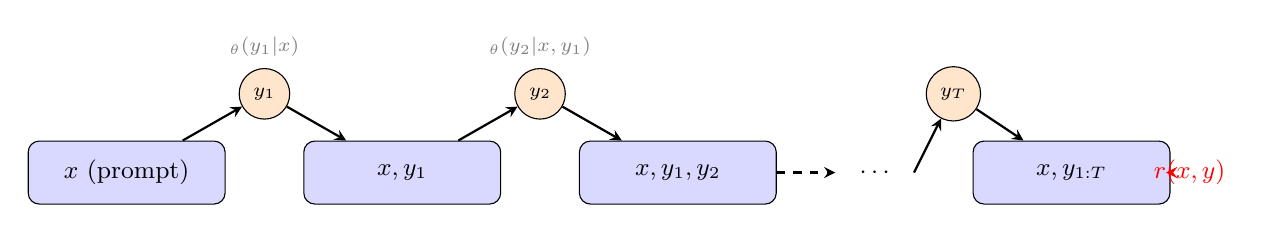
\begin{tikzpicture}[
        state/.style={draw, rounded corners, fill=blue!15, minimum width=2.5cm, minimum height=0.8cm, align=center, font=\small},
        action/.style={circle, draw, fill=orange!20, minimum size=0.6cm, font=\scriptsize},
        arrow/.style={->, thick, >=stealth}
    ]
        % 状态序列
        \node[state] (s0) at (0, 0) {$x$ (prompt)};
        \node[state] (s1) at (3.5, 0) {$x, y_1$};
        \node[state] (s2) at (7, 0) {$x, y_1, y_2$};
        \node[font=\small] at (9.5, 0) {$\cdots$};
        \node[state] (sT) at (12, 0) {$x, y_{1:T}$};

        % 动作
        \node[action] (a1) at (1.75, 1) {$y_1$};
        \node[action] (a2) at (5.25, 1) {$y_2$};
        \node[action] (aT) at (10.5, 1) {$y_T$};

        % 奖励
        \node[font=\small, red] at (13.5, 0) {$r(x, y)$};

        % 连接
        \draw[arrow] (s0) -- (a1);
        \draw[arrow] (a1) -- (s1);
        \draw[arrow] (s1) -- (a2);
        \draw[arrow] (a2) -- (s2);
        \draw[arrow, dashed] (s2) -- (9, 0);
        \draw[arrow] (10, 0) -- (aT);
        \draw[arrow] (aT) -- (sT);
        \draw[arrow, red] (sT) -- (13.2, 0);

        % 标注
        \node[font=\scriptsize, gray] at (1.75, 1.6) {$\policy_\theta(y_1|x)$};
        \node[font=\scriptsize, gray] at (5.25, 1.6) {$\policy_\theta(y_2|x,y_1)$};
    \end{tikzpicture}
    \caption{LLM 生成过程的 MDP 建模}
    \label{fig:llm-mdp}
\end{figure}

LLM RL 的特点:
\begin{itemize}
    \item \textbf{动作空间巨大}:词表通常有 10 万+ token
    \item \textbf{确定性状态转移}:下一状态 = 当前状态 + 新 token
    \item \textbf{Episode = 一次完整生成}:从 prompt 到 EOS
    \item \textbf{稀疏奖励}:只有序列结束时才有奖励信号
\end{itemize}

\subsection{稀疏奖励问题}

LLM 对齐的典型奖励结构:
\begin{equation}
    r_t = \begin{cases}
        0 & t < T \\
        r_\phi(x, y) & t = T \text{(序列结束)}
    \end{cases}
\end{equation}

稀疏奖励带来的挑战:
\begin{itemize}
    \item \textbf{信用分配困难}:最终奖励如何归因到每个 token?
    \item \textbf{梯度信号弱}:大部分时刻没有学习信号
    \item \textbf{长序列尤其困难}:信号需要传播很远(数千 token)
\end{itemize}

\begin{note}
解决稀疏奖励的两种思路:
\begin{enumerate}
    \item \textbf{序列级方法}:把整个序列当作一个 bandit,用序列奖励直接更新(如 REINFORCE)
    \item \textbf{过程奖励}:训练 PRM 提供中间步骤的奖励信号
\end{enumerate}
\end{note}

% ------------------------------------------
\section{RLHF 三阶段}
\label{sec:rlhf}

RLHF(Reinforcement Learning from Human Feedback)是 LLM 对齐的经典方法,由 OpenAI 在 InstructGPT 中系统化。

\subsection{RLHF 整体架构}

\begin{figure}[H]
    \centering
    \begin{tikzpicture}[scale=0.9, every node/.style={scale=0.9},
        box/.style={draw, rounded corners, minimum width=2.8cm, minimum height=1cm, align=center},
        data/.style={draw, rounded corners, fill=gray!15, minimum width=2cm, minimum height=0.8cm, align=center, font=\small},
        arrow/.style={->, thick, >=stealth}
    ]
        % Stage 1
        \begin{scope}[shift={(-5, 0)}]
            \node[box, fill=blue!20] (pt) at (0, 2) {预训练模型};
            \node[data] (sft_data) at (0, 0) {高质量对话\\数据};
            \node[box, fill=green!20] (sft) at (0, -2) {SFT 模型\\$\policy_{\text{ref}}$};

            \draw[arrow] (pt) -- (sft);
            \draw[arrow] (sft_data) -- (sft);

            \node[font=\bfseries] at (0, 3.5) {Stage 1: SFT};
        \end{scope}

        % Stage 2
        \begin{scope}[shift={(0, 0)}]
            \node[box, fill=green!15] (sft2) at (0, 2) {SFT 模型};
            \node[data] (pref_data) at (0, 0) {人类偏好数据\\$(x, y_w, y_l)$};
            \node[box, fill=orange!20] (rm) at (0, -2) {Reward Model\\$r_\phi(x, y)$};

            \draw[arrow] (sft2) -- (rm);
            \draw[arrow] (pref_data) -- (rm);

            \node[font=\bfseries] at (0, 3.5) {Stage 2: RM};
        \end{scope}

        % Stage 3
        \begin{scope}[shift={(5.5, 0)}]
            \node[box, fill=green!15] (ref) at (-1.8, 2) {$\policy_{\text{ref}}$};
            \node[box, fill=orange!15] (rm2) at (1.8, 2) {$r_\phi$};
            \node[box, fill=purple!20] (ppo) at (0, 0) {PPO 训练};
            \node[box, fill=red!20] (final) at (0, -2) {对齐模型\\$\policy_\theta$};

            \draw[arrow] (ref) -- (ppo);
            \draw[arrow] (rm2) -- (ppo);
            \draw[arrow] (ppo) -- (final);

            \node[font=\bfseries] at (0, 3.5) {Stage 3: PPO};
        \end{scope}

        % 连接箭头
        \draw[arrow, dashed, gray] (-3, -2) -- (-2, 2);
        \draw[arrow, dashed, gray] (2, -2) -- (4, 2);
    \end{tikzpicture}
    \caption{RLHF 三阶段架构}
    \label{fig:rlhf-pipeline}
\end{figure}

\subsection{Stage 1: Supervised Fine-Tuning (SFT)}

用高质量对话数据微调预训练模型:
\begin{equation}
    L_{\text{SFT}}(\theta) = -\E_{(x,y) \sim \mathcal{D}_{\text{SFT}}} \left[ \log \policy_\theta(y|x) \right] = -\E \left[ \sum_{t=1}^{T} \log \policy_\theta(y_t | x, y_{<t}) \right]
\end{equation}

SFT 的作用:
\begin{itemize}
    \item 让模型学会"指令遵循"的基本格式
    \item 提供 RL 的起点(参考模型 $\policy_{\text{ref}}$)
    \item 过滤预训练中的低质量模式
\end{itemize}

\subsection{Stage 2: Reward Model 训练}

从人类偏好数据中学习 Reward Model。

\begin{definition}[偏好数据]
对于 prompt $x$,人类标注者比较两个回复,给出偏好:$y_w \succ y_l$($y_w$ 优于 $y_l$)。
\end{definition}

\subsubsection{Bradley-Terry 模型}

\begin{definition}[Bradley-Terry 模型]
假设人类偏好遵循 Bradley-Terry 模型——偏好概率由"能力差"决定:
\begin{equation}
    P(y_w \succ y_l | x) = \sigma(r(x, y_w) - r(x, y_l)) = \frac{1}{1 + e^{-(r(x, y_w) - r(x, y_l))}}
    \label{eq:bradley-terry}
\end{equation}
其中 $\sigma(z) = \frac{1}{1+e^{-z}}$ 是 sigmoid 函数,$r(x, y)$ 是回复的"得分"。
\end{definition}

\begin{figure}[H]
    \centering
    \begin{tikzpicture}
        \begin{axis}[
            width=10cm, height=5cm,
            xlabel={$r(y_w) - r(y_l)$(奖励差)},
            ylabel={$P(y_w \succ y_l)$(偏好概率)},
            domain=-6:6,
            samples=100,
            grid=major,
            ymin=0, ymax=1
        ]
            \addplot[thick, blue] {1/(1+exp(-x))};
            \draw[dashed, gray] (axis cs:0, 0.5) -- (axis cs:0, 0);
            \node[font=\small] at (axis cs:3, 0.3) {奖励差越大};
            \node[font=\small] at (axis cs:3, 0.2) {偏好越确定};
        \end{axis}
    \end{tikzpicture}
    \caption{Bradley-Terry 模型:偏好概率由奖励差决定}
    \label{fig:bradley-terry}
\end{figure}

Bradley-Terry 模型的直觉:
\begin{itemize}
    \item 奖励差 = 0 时,偏好概率 = 0.5(无法区分)
    \item 奖励差越大,偏好概率越接近 1(更确定)
    \item 模型假设偏好是基于"内在质量分数"的概率比较
\end{itemize}

\subsubsection{Reward Model 训练}

Reward Model 的训练目标是最大化偏好数据的似然:
\begin{equation}
    L_{\text{RM}}(\phi) = -\E_{(x, y_w, y_l)} \left[ \log \sigma(r_\phi(x, y_w) - r_\phi(x, y_l)) \right]
    \label{eq:rm-loss}
\end{equation}

这是一个\textbf{二分类问题}:给定 $(y_w, y_l)$,预测哪个更好。

\begin{note}
Reward Model 的架构选择:
\begin{itemize}
    \item 通常用 SFT 模型初始化
    \item 去掉语言模型头,加上标量输出头
    \item 输入 $(x, y)$,输出标量 $r_\phi(x, y) \in \R$
\end{itemize}
\end{note}

\subsection{Stage 3: PPO 微调}

使用 Reward Model 提供奖励信号,用 PPO 优化策略。

\begin{definition}[RLHF 优化目标]
\begin{equation}
    \max_\theta \E_{x \sim \mathcal{D}, y \sim \policy_\theta(\cdot|x)} \left[ r_\phi(x, y) \right] - \beta \cdot \text{KL}(\policy_\theta \| \policy_{\text{ref}})
    \label{eq:rlhf-objective}
\end{equation}
其中 $\beta > 0$ 是 KL 正则系数。
\end{definition}

\subsubsection{KL 正则的作用}

KL 正则项 $\text{KL}(\policy_\theta \| \policy_{\text{ref}})$ 至关重要:

\begin{enumerate}
    \item \textbf{防止 Reward Hacking}:
    \begin{itemize}
        \item Reward Model 是不完美的代理
        \item 无约束优化会找到"欺骗" RM 的方式
        \item 例如:生成特定模式获得高分,但实际质量差
    \end{itemize}

    \item \textbf{保持生成质量}:
    \begin{itemize}
        \item SFT 模型已经有较好的语言能力
        \item KL 约束防止偏离太远导致流利度下降
    \end{itemize}

    \item \textbf{稳定训练}:
    \begin{itemize}
        \item 约束优化空间,避免策略崩溃
        \item 提供正则化效果
    \end{itemize}
\end{enumerate}

\begin{figure}[H]
    \centering
    \begin{tikzpicture}[
        arrow/.style={->, thick, >=stealth}
    ]
        % 坐标轴
        \draw[arrow] (-0.5, 0) -- (8, 0) node[right] {$\text{KL}(\policy_\theta \| \policy_{\text{ref}})$};
        \draw[arrow] (0, -0.5) -- (0, 5) node[above] {$\E[r_\phi]$};

        % 曲线
        \draw[thick, blue, domain=0.2:7, samples=100] plot (\x, {4 - 0.8*(\x-3)^2/9 + 0.5*ln(\x)});

        % 最优点
        \fill[red] (2.5, 3.8) circle (3pt);
        \node[font=\small, red] at (2.5, 4.3) {最优权衡};

        % 区域标注
        \node[font=\scriptsize, align=center] at (1, 2) {KL 太小\\改进有限};
        \node[font=\scriptsize, align=center] at (6, 2) {KL 太大\\Reward Hacking};

        % beta 的作用
        \draw[dashed, gray] (0, 3.8) -- (2.5, 3.8) -- (2.5, 0);
    \end{tikzpicture}
    \caption{KL 正则的权衡:$\beta$ 控制在 reward 和 KL 之间的平衡点}
    \label{fig:kl-tradeoff}
\end{figure}

\subsubsection{PPO 更新流程}

RLHF 中 PPO 的具体步骤:

\begin{algorithm}[H]
\caption{RLHF with PPO}
\label{alg:rlhf-ppo}
\KwInput{SFT 模型 $\policy_{\text{ref}}$,Reward Model $r_\phi$,KL 系数 $\beta$}
初始化 $\policy_\theta \leftarrow \policy_{\text{ref}}$,Critic $\Val_\psi$\;
\ForEach{iteration}{
    \tcp{采样}
    从 prompt 分布采样 $x \sim \mathcal{D}$\;
    用当前策略生成回复 $y \sim \policy_\theta(\cdot|x)$\;

    \tcp{计算奖励}
    计算 RM 奖励:$r^{\text{RM}} = r_\phi(x, y)$\;
    计算 KL 惩罚:$r^{\text{KL}}_t = -\beta \log \frac{\policy_\theta(y_t|x, y_{<t})}{\policy_{\text{ref}}(y_t|x, y_{<t})}$\;
    总奖励:$r_t = r^{\text{KL}}_t + \ind_{t=T} \cdot r^{\text{RM}}$\;

    \tcp{GAE 计算}
    用 Critic $\Val_\psi$ 计算 advantage $\hat{\advantage}_t$\;

    \tcp{PPO 更新}
    用 PPO-Clip 目标更新 $\policy_\theta$\;
    用 TD 目标更新 $\Val_\psi$\;
}
\end{algorithm}

\begin{important}
RLHF 需要维护的模型:
\begin{enumerate}
    \item $\policy_\theta$:正在训练的策略(Active Model)
    \item $\policy_{\text{ref}}$:参考模型(冻结)
    \item $r_\phi$:Reward Model(冻结)
    \item $\Val_\psi$:Critic 网络
\end{enumerate}
共 4 个大模型,显存开销巨大!这是 DPO、GRPO 等方法试图解决的问题。
\end{important}

% ------------------------------------------
\section{Direct Preference Optimization (DPO)}
\label{sec:dpo}

DPO 是一种绕过 Reward Model 和 PPO 的简化方法,由 Rafailov et al. 2023 提出。

\subsection{DPO 的动机}

RLHF + PPO 的问题:
\begin{itemize}
    \item \textbf{模型开销大}:需要维护 4 个模型
    \item \textbf{采样成本高}:大模型在线生成很贵
    \item \textbf{实现复杂}:PPO 超参敏感,需要精细调参
    \item \textbf{训练不稳定}:RL 训练容易崩溃
\end{itemize}

\begin{quote}
\textbf{DPO 的核心问题}:能否直接在偏好数据 $(x, y_w, y_l)$ 上优化,像监督学习一样简单?
\end{quote}

答案是可以的!关键洞察:KL 正则的 RL 问题有\textbf{闭式解}。

\subsection{DPO Loss 公式}

\begin{definition}[DPO Loss]
\begin{equation}
    L_{\text{DPO}}(\theta) = -\E_{(x, y_w, y_l)} \left[ \log \sigma \left( \beta \left[ \log \frac{\policy_\theta(y_w|x)}{\policy_{\text{ref}}(y_w|x)} - \log \frac{\policy_\theta(y_l|x)}{\policy_{\text{ref}}(y_l|x)} \right] \right) \right]
    \label{eq:dpo-loss}
\end{equation}
\end{definition}

\subsection{DPO 完整推导}

\begin{theorem}[DPO 等价性]
DPO Loss \eqref{eq:dpo-loss} 与 RLHF 目标 \eqref{eq:rlhf-objective} 在最优解处等价。
\end{theorem}

\begin{proof}
推导分为 5 个关键步骤。

\textbf{Step 1:RLHF 目标展开}

RLHF 优化目标:
\begin{equation}
    \max_\policy \E_{y \sim \policy} \left[ r(x, y) \right] - \beta \cdot \text{KL}(\policy \| \policy_{\text{ref}})
\end{equation}

展开 KL 散度:
\begin{align}
    &= \E_{y \sim \policy} \left[ r(x, y) \right] - \beta \E_{y \sim \policy} \left[ \log \frac{\policy(y|x)}{\policy_{\text{ref}}(y|x)} \right] \\
    &= \E_{y \sim \policy} \left[ r(x, y) - \beta \log \frac{\policy(y|x)}{\policy_{\text{ref}}(y|x)} \right]
\end{align}

\textbf{Step 2:引入配分函数 $Z(x)$}

为了让最优策略是合法的概率分布,定义配分函数:
\begin{equation}
    Z(x) = \sum_y \policy_{\text{ref}}(y|x) \exp\left( \frac{r(x,y)}{\beta} \right)
\end{equation}

$Z(x)$ 是归一化常数,只依赖于 $x$(不依赖于被优化的策略)。

\textbf{Step 3:最优策略的闭式解}

KL 正则 RL 问题有闭式解:

\begin{lemma}[KL 正则 RL 的最优策略]
目标 $\max_\policy \E_{y \sim \policy}[r(y)] - \beta \cdot \text{KL}(\policy \| \policy_{\text{ref}})$ 的最优解为:
\begin{equation}
    \policy^*(y|x) = \frac{1}{Z(x)} \policy_{\text{ref}}(y|x) \exp\left( \frac{r(x,y)}{\beta} \right)
    \label{eq:optimal-policy-kl}
\end{equation}
\end{lemma}

\begin{proof}
这是一个有约束优化问题($\policy$ 需要是概率分布)。用拉格朗日乘子法或变分推断可得。
直觉:最优策略是参考策略按 $\exp(r/\beta)$ 重新加权。奖励越高,概率提升越多。
\end{proof}

\textbf{Step 4:从最优策略反解 reward}

关键步骤:从 \eqref{eq:optimal-policy-kl} 反解 reward。

取对数:
\begin{align}
    \log \policy^*(y|x) &= \log \policy_{\text{ref}}(y|x) - \log Z(x) + \frac{r(x,y)}{\beta}
\end{align}

整理得:
\begin{equation}
    r(x,y) = \beta \log \frac{\policy^*(y|x)}{\policy_{\text{ref}}(y|x)} + \beta \log Z(x)
    \label{eq:reward-from-policy}
\end{equation}

\begin{keypoint}
核心洞察:reward 可以用策略的 log-ratio 表示!虽然有 $\log Z(x)$ 项,但它只依赖于 $x$,在 pairwise 比较中会消除。
\end{keypoint}

\textbf{Step 5:代入 Bradley-Terry 模型,$Z(x)$ 消除}

将 \eqref{eq:reward-from-policy} 代入 Bradley-Terry 模型 \eqref{eq:bradley-terry}:
\begin{align}
    P(y_w \succ y_l) &= \sigma(r(x, y_w) - r(x, y_l)) \\
    &= \sigma\bigg( \underbrace{\beta \log \frac{\policy^*(y_w|x)}{\policy_{\text{ref}}(y_w|x)} + \beta \log Z(x)}_{r(x, y_w)} - \underbrace{\beta \log \frac{\policy^*(y_l|x)}{\policy_{\text{ref}}(y_l|x)} - \beta \log Z(x)}_{r(x, y_l)} \bigg) \\
    &= \sigma\left( \beta \left[ \log \frac{\policy^*(y_w|x)}{\policy_{\text{ref}}(y_w|x)} - \log \frac{\policy^*(y_l|x)}{\policy_{\text{ref}}(y_l|x)} \right] \right)
\end{align}

$\beta \log Z(x)$ 项相消了!

最大化偏好数据的 log-likelihood,用 $\policy_\theta$ 代替 $\policy^*$,得到 DPO Loss:
\begin{equation}
    L_{\text{DPO}}(\theta) = -\E \left[ \log \sigma \left( \beta \left[ \log \frac{\policy_\theta(y_w|x)}{\policy_{\text{ref}}(y_w|x)} - \log \frac{\policy_\theta(y_l|x)}{\policy_{\text{ref}}(y_l|x)} \right] \right) \right]
\end{equation}
\end{proof}

\begin{figure}[H]
    \centering
    \begin{tikzpicture}[
        box/.style={draw, rounded corners, fill=blue!10, minimum width=3.5cm, minimum height=1cm, align=center},
        arrow/.style={->, thick, >=stealth}
    ]
        \node[box] (rlhf) at (0, 3) {RLHF 目标\\$\max \E[r] - \beta \cdot \text{KL}$};
        \node[box] (opt) at (0, 1) {最优策略闭式解\\$\policy^* \propto \policy_{\text{ref}} \exp(r/\beta)$};
        \node[box] (reward) at (0, -1) {反解 reward\\$r = \beta \log \frac{\policy^*}{\policy_{\text{ref}}} + \beta \log Z$};
        \node[box, fill=green!20] (dpo) at (0, -3) {DPO Loss\\$Z(x)$ 消除};

        \draw[arrow] (rlhf) -- node[right, font=\small] {KL-RL 闭式解} (opt);
        \draw[arrow] (opt) -- node[right, font=\small] {取对数} (reward);
        \draw[arrow] (reward) -- node[right, font=\small] {代入 BT 模型} (dpo);
    \end{tikzpicture}
    \caption{DPO 推导的逻辑链条}
    \label{fig:dpo-derivation}
\end{figure}

\begin{important}
DPO 的核心洞察:
\begin{enumerate}
    \item KL 正则 RL 问题有闭式解,最优策略是参考策略的指数重加权
    \item 可以从最优策略反解隐式 reward
    \item 配分函数 $Z(x)$ 在 pairwise 比较中消除——这是 DPO 能 work 的关键
    \item 最终形式只需要计算 log-probability,像监督学习一样简单
\end{enumerate}
\end{important}

\subsection{DPO 的直观理解}

定义 \textbf{隐式奖励}:
\begin{equation}
    \hat{r}_\theta(x, y) = \beta \log \frac{\policy_\theta(y|x)}{\policy_{\text{ref}}(y|x)}
\end{equation}

DPO Loss 可以写成:
\begin{equation}
    L_{\text{DPO}} = -\E \left[ \log \sigma(\hat{r}_\theta(x, y_w) - \hat{r}_\theta(x, y_l)) \right]
\end{equation}

直觉:
\begin{itemize}
    \item $\hat{r}_\theta(x, y_w) > \hat{r}_\theta(x, y_l)$:$y_w$ 的隐式奖励更高,loss 变小
    \item 训练过程提高 $y_w$ 相对于 $\policy_{\text{ref}}$ 的概率,压低 $y_l$ 的概率
    \item $\beta$ 控制"相对于参考策略偏离多少"的尺度
\end{itemize}

\subsection{DPO vs RLHF 对比}

\begin{table}[H]
    \centering
    \begin{tabular}{@{}lcc@{}}
        \toprule
        & \textbf{RLHF + PPO} & \textbf{DPO} \\
        \midrule
        需要 Reward Model & 是 & 否 \\
        需要 Critic 网络 & 是 & 否 \\
        训练方式 & 在线采样 & 离线训练 \\
        模型数量 & 4 个 & 2 个 \\
        实现复杂度 & 高 & 低 \\
        超参敏感性 & 高 & 低 \\
        探索能力 & 有 & 无 \\
        适用场景 & 复杂任务 & 简单对齐 \\
        \bottomrule
    \end{tabular}
    \caption{RLHF + PPO 与 DPO 的对比}
\end{table}

DPO 的局限:
\begin{itemize}
    \item \textbf{无探索}:完全离线,只能在已有偏好数据的分布内优化
    \item \textbf{Pairwise 信号粗糙}:只知道谁更好,不知道好多少
    \item \textbf{难任务提升有限}:在数学、代码等需要探索的任务上效果不如 RL
\end{itemize}

% ------------------------------------------
\section{GRPO:Group Relative Policy Optimization}
\label{sec:grpo}

GRPO 是 DeepSeek 提出的方法,介于 PPO 和 DPO 之间:保留在线探索能力,但不需要 Critic 网络。

\subsection{GRPO 的动机}

\begin{itemize}
    \item \textbf{PPO 的问题}:需要 Critic 网络,显存开销大(额外一个大模型)
    \item \textbf{DPO 的问题}:完全离线,缺乏探索,难任务提升有限
\end{itemize}

GRPO 的思路:\textbf{用组内相对奖励代替 Critic},实现"无 Critic 的在线 RL"。

\subsection{组内标准化 Advantage}

\begin{definition}[GRPO Advantage]
对于 prompt $x$,采样一组回复 $\{y_1, \ldots, y_G\}$,计算各自的奖励 $\{R_1, \ldots, R_G\}$,然后:
\begin{equation}
    \hat{\advantage}_i = \frac{R_i - \bar{R}}{\text{Std}(R) + \epsilon}
    \label{eq:grpo-advantage}
\end{equation}
其中 $\bar{R} = \frac{1}{G}\sum_i R_i$ 是组内均值,$\text{Std}(R)$ 是组内标准差。
\end{definition}

\begin{figure}[H]
    \centering
    \begin{tikzpicture}[
        sample/.style={circle, draw, minimum size=0.6cm, font=\scriptsize},
        arrow/.style={->, thick, >=stealth}
    ]
        % Prompt
        \node[draw, rounded corners, fill=blue!20, minimum width=2cm] (prompt) at (0, 0) {Prompt $x$};

        % 生成多个回复
        \node[sample, fill=green!30] (y1) at (3, 1.5) {$y_1$};
        \node[sample, fill=green!20] (y2) at (3, 0.5) {$y_2$};
        \node[sample, fill=red!20] (y3) at (3, -0.5) {$y_3$};
        \node[sample, fill=red!30] (y4) at (3, -1.5) {$y_4$};

        \draw[arrow] (prompt) -- (y1);
        \draw[arrow] (prompt) -- (y2);
        \draw[arrow] (prompt) -- (y3);
        \draw[arrow] (prompt) -- (y4);

        % 奖励
        \node[font=\scriptsize] at (4.5, 1.5) {$R_1 = 0.8$};
        \node[font=\scriptsize] at (4.5, 0.5) {$R_2 = 0.6$};
        \node[font=\scriptsize] at (4.5, -0.5) {$R_3 = 0.3$};
        \node[font=\scriptsize] at (4.5, -1.5) {$R_4 = 0.1$};

        % 标准化
        \node[font=\small] at (7, 0) {$\bar{R} = 0.45$};

        % Advantage
        \node[font=\scriptsize, green!60!black] at (9, 1.5) {$\hat{A}_1 > 0$};
        \node[font=\scriptsize, green!60!black] at (9, 0.5) {$\hat{A}_2 > 0$};
        \node[font=\scriptsize, red] at (9, -0.5) {$\hat{A}_3 < 0$};
        \node[font=\scriptsize, red] at (9, -1.5) {$\hat{A}_4 < 0$};

        % 说明
        \node[font=\small, align=center] at (5, -3) {组内相对比较:\\高于均值的增强,低于均值的抑制};
    \end{tikzpicture}
    \caption{GRPO 组内标准化示意图}
    \label{fig:grpo-advantage}
\end{figure}

组内标准化的优势:
\begin{enumerate}
    \item \textbf{无需 Critic}:用组内均值代替价值函数估计
    \item \textbf{Baseline 效果}:均值减法降低方差
    \item \textbf{尺度归一化}:标准差归一化使 advantage 尺度稳定
    \item \textbf{相对比较}:focus 在同一 prompt 下的相对好坏
\end{enumerate}

\subsection{GRPO 目标函数}

\begin{definition}[GRPO 目标]
\begin{equation}
    L_{\text{GRPO}} = \E_{x} \left[ \frac{1}{G} \sum_{i=1}^{G} \sum_{t=1}^{|y_i|} \min \left( \rho_{i,t} \hat{\advantage}_i, \text{clip}(\rho_{i,t}, 1-\epsilon, 1+\epsilon) \hat{\advantage}_i \right) \right]
\end{equation}
其中 $\rho_{i,t} = \frac{\policy_\theta(y_{i,t}|x, y_{i,<t})}{\policy_{\theta_{\text{old}}}(y_{i,t}|x, y_{i,<t})}$ 是 importance sampling 比率。
\end{definition}

\begin{note}
GRPO 与 PPO 的关键区别:
\begin{itemize}
    \item PPO:$\hat{\advantage}_t$ 由 GAE 计算,需要 Critic
    \item GRPO:$\hat{\advantage}_i$ 对整个序列恒定,由组内标准化得到
\end{itemize}
\end{note}

\subsection{GRPO 实用技巧}

\begin{enumerate}
    \item \textbf{Clip-Higher}:上界可以更宽松(如 $1+0.28$ 而非 $1+0.2$),允许好回复更大幅度提升

    \item \textbf{Dynamic Sampling}:过滤全对或全错的 prompt(方差为 0 时 advantage 无定义)

    \item \textbf{长度惩罚}:防止生成过长的回复
    \begin{equation}
        R_i = r_\phi(x, y_i) - \lambda \cdot |y_i|
    \end{equation}

    \item \textbf{KL as Loss}:KL 惩罚作为独立 loss 项,而非放入 reward
    \begin{equation}
        L = -L_{\text{GRPO}} + \lambda_{\text{KL}} \cdot \E[\text{KL}(\policy_\theta \| \policy_{\text{ref}})]
    \end{equation}
\end{enumerate}

% ------------------------------------------
\section{KL 散度估计:k1, k2, k3}
\label{sec:kl-estimators}

KL 散度 $\text{KL}(\policy_\theta \| \policy_{\text{ref}})$ 无法精确计算(需要遍历所有可能的序列),需要蒙特卡洛估计。

\subsection{KL 散度的定义}

对于两个分布 $p$ 和 $q$:
\begin{equation}
    \text{KL}(p \| q) = \E_{x \sim p}\left[ \log \frac{p(x)}{q(x)} \right]
\end{equation}

在 LLM 场景中,$p = \policy_\theta$,$q = \policy_{\text{ref}}$,从 $\policy_\theta$ 采样。

\subsection{k1 估计器:直接估计}

\begin{definition}[k1 估计器]
定义比率 $r = \frac{\policy_{\text{ref}}(y|x)}{\policy_\theta(y|x)}$,则:
\begin{equation}
    k_1 = -\log r = \log \frac{\policy_\theta(y|x)}{\policy_{\text{ref}}(y|x)}
\end{equation}
\end{definition}

性质:
\begin{itemize}
    \item \textbf{无偏}:$\E_{y \sim \policy_\theta}[k_1] = \text{KL}(\policy_\theta \| \policy_{\text{ref}})$
    \item \textbf{高方差}:当 $\policy_\theta$ 和 $\policy_{\text{ref}}$ 差异大时,方差很大
\end{itemize}

用法:通常放入 reward
\begin{equation}
    r_t^{\text{RL}} = r_t^{\text{RM}} - \beta \cdot k_1^{(t)}
\end{equation}

\subsection{k2 估计器:平方形式}

\begin{definition}[k2 估计器]
\begin{equation}
    k_2 = \frac{1}{2}(\log r)^2 = \frac{1}{2} \left( \log \frac{\policy_{\text{ref}}(y|x)}{\policy_\theta(y|x)} \right)^2
\end{equation}
\end{definition}

性质:
\begin{itemize}
    \item \textbf{有偏}:$\E[k_2] \neq \text{KL}$
    \item \textbf{梯度等价}:$\nabla_\theta \E[k_2] = \nabla_\theta \text{KL}$
    \item \textbf{更平滑}:平方形式在 $r=1$ 附近更平滑
\end{itemize}

用法:适合作为 loss 项(因为梯度正确)

\subsection{k3 估计器:Control Variate}

\begin{definition}[k3 估计器]
\begin{equation}
    k_3 = (r - 1) - \log r = \frac{\policy_{\text{ref}}(y|x)}{\policy_\theta(y|x)} - 1 - \log \frac{\policy_{\text{ref}}(y|x)}{\policy_\theta(y|x)}
\end{equation}
\end{definition}

\begin{theorem}[k3 的性质]
k3 是无偏且低方差的 KL 估计器。
\end{theorem}

\begin{proof}
无偏性:
\begin{align}
    \E_{y \sim \policy_\theta}[k_3] &= \E[(r-1)] - \E[\log r] \\
    &= \underbrace{\E\left[\frac{\policy_{\text{ref}}}{\policy_\theta}\right] - 1}_{= 0} + \E\left[\log \frac{\policy_\theta}{\policy_{\text{ref}}}\right] \\
    &= \text{KL}(\policy_\theta \| \policy_{\text{ref}})
\end{align}

其中 $\E_{y \sim \policy_\theta}\left[\frac{\policy_{\text{ref}}(y)}{\policy_\theta(y)}\right] = \sum_y \policy_\theta(y) \cdot \frac{\policy_{\text{ref}}(y)}{\policy_\theta(y)} = \sum_y \policy_{\text{ref}}(y) = 1$。

低方差:$(r-1)$ 项是一个 control variate,期望为 0,与 $\log r$ 负相关,减少方差。
\end{proof}

\subsection{三种估计器对比}

\begin{table}[H]
    \centering
    \begin{tabular}{@{}lcccc@{}}
        \toprule
        估计器 & 公式 & 偏差 & 方差 & 推荐用法 \\
        \midrule
        k1 & $\log \frac{\policy_\theta}{\policy_{\text{ref}}}$ & 无偏 & 高 & KL in reward \\
        k2 & $\frac{1}{2}(\log \frac{\policy_{\text{ref}}}{\policy_\theta})^2$ & 有偏 & 低 & KL as loss \\
        k3 & $\frac{\policy_{\text{ref}}}{\policy_\theta} - 1 - \log \frac{\policy_{\text{ref}}}{\policy_\theta}$ & 无偏 & 低 & KL as loss \\
        \bottomrule
    \end{tabular}
    \caption{KL 估计器对比}
\end{table}

\begin{keypoint}
KL 的两种用法:
\begin{enumerate}
    \item \textbf{KL in Reward}(经典 RLHF):
    \begin{itemize}
        \item Token reward 减去 $\beta \cdot k_1$
        \item 然后用 PPO-Clip 更新
        \item 优点:直接影响每步决策
    \end{itemize}

    \item \textbf{KL as Loss}(GRPO 等):
    \begin{itemize}
        \item 总 loss = $-L_{\text{RL}} + \lambda \cdot \E[k_3]$
        \item 优点:更稳定,方差更低
    \end{itemize}
\end{enumerate}
\end{keypoint}

% ------------------------------------------
\section{On-Policy Distillation}
\label{sec:on-policy-distillation}

On-Policy Distillation 是近年来 LLM 后训练的重要进展,由 GKD~\cite{agarwal2024gkd} 和 MiniLLM~\cite{gu2024minillm} 等工作奠定基础,并在 Qwen3~\cite{yang2025qwen3} 等前沿模型中得到成功应用。

\subsection{动机:Off-policy 蒸馏的分布偏移问题}

传统的知识蒸馏(SFT on 教师数据)是 \textbf{off-policy} 的:

\begin{quote}
\textbf{学生从教师生成的数据学习,但推理时走到的状态可能与训练时完全不同。}
\end{quote}

这导致 \textbf{compounding errors}——学生在训练时没见过自己犯的错误,一旦偏离教师轨迹就会持续恶化。尤其在长序列推理任务中,这种分布偏移问题更为严重。

\begin{itemize}
    \item \textbf{Off-policy SFT}:密集监督,但分布偏移
    \item \textbf{On-policy RL}:分布匹配,但奖励稀疏、效率低
\end{itemize}

自然的问题:能否结合两者优势——在学生自己的分布上获得密集监督?

\subsection{三种后训练范式对比}

\begin{table}[H]
    \centering
    \begin{tabular}{@{}lccc@{}}
        \toprule
        方法 & 采样来源 & 奖励密度 & 特点 \\
        \midrule
        SFT(监督微调) & 教师数据(Off-policy) & 密集 & 分布受限 \\
        RL(强化学习) & 自身采样(On-policy) & 稀疏 & 搜索成本高 \\
        On-Policy Distillation & \textbf{自身采样} & \textbf{密集} & 两者优势结合 \\
        \bottomrule
    \end{tabular}
    \caption{三种后训练范式对比}
    \label{tab:post-training-paradigms}
\end{table}

On-Policy Distillation 的核心思想:
\begin{itemize}
    \item \textbf{学生自己采样}(On-policy):避免分布偏移
    \item \textbf{教师逐 token 打分}(Dense reward):提供密集监督信号
\end{itemize}

\subsection{Reverse KL 损失}

On-Policy Distillation 使用 \textbf{反向 KL 散度}作为损失函数:
\begin{equation}
    L_{\text{OPD}} = D_{\text{KL}}(\policy_\theta \| \policy_{\text{teacher}}) = \E_{y \sim \policy_\theta}\left[ \sum_t \log \frac{\policy_\theta(y_t | x, y_{<t})}{\policy_{\text{teacher}}(y_t | x, y_{<t})} \right]
\end{equation}

\begin{note}
\textbf{Forward KL vs Reverse KL}:
\begin{itemize}
    \item Forward KL $D_{\text{KL}}(\policy_{\text{teacher}} \| \policy_\theta)$:mode covering,学生试图覆盖教师的所有模式
    \item Reverse KL $D_{\text{KL}}(\policy_\theta \| \policy_{\text{teacher}})$:mode seeking,学生专注于教师的高概率区域
\end{itemize}
Reverse KL 更适合蒸馏场景——让学生在自己访问的状态上模仿教师,而非试图覆盖教师的全部行为。
\end{note}

\subsection{KDRL:结合知识蒸馏与强化学习}

KDRL~\cite{xu2025kdrl}(Knowledge Distillation + Reinforcement Learning)将教师监督和奖励驱动的自我探索统一为联合优化:

\begin{equation}
    \mathcal{J}_{\text{KDRL}}(\theta) = \underbrace{\mathcal{J}_{\text{GRPO}}(\theta)}_{\text{奖励驱动}} - \beta \cdot \underbrace{D_{\text{KL}}^{k_2}(\policy_\theta \| \policy_{\text{teacher}})}_{\text{教师监督}}
\end{equation}

关键设计选择:
\begin{enumerate}
    \item \textbf{KL 估计器选择}:$k_2$ 优于 $k_3$,因为 $k_2$ 提供无偏梯度估计
    \item \textbf{系数退火}:从强模仿($\beta$ 大)逐渐过渡到奖励驱动($\beta$ 小)
    \item \textbf{奖励引导 Masking}:只在低奖励样本上应用 KD,减少输出长度同时保持准确率
\end{enumerate}

\subsection{效率优势}

\begin{keypoint}
On-Policy Distillation 的效率提升(以数学推理任务为例):
\begin{itemize}
    \item 相比 RL:训练速度快 7-10 倍,总计算效率提升 50-100 倍
    \item 相比离线蒸馏:计算成本降低 9-30 倍
    \item Qwen3 实验:蒸馏显著优于 RL,GPU 小时仅需 RL 的约 1/10
\end{itemize}
\end{keypoint}

效率提升的根本原因:
\begin{quote}
\textbf{教师提供的密集 token 级信号,比 RL 的稀疏序列级奖励包含更多信息。}

RL 的大部分计算花在搜索(探索策略空间),蒸馏则直接利用教师的知识指导学生在关键"分叉点"做出正确选择。
\end{quote}

\subsection{应用场景}

\begin{enumerate}
    \item \textbf{小模型专业化}:用大模型(如 Qwen3-235B)蒸馏小模型(如 Qwen3-32B)
    \item \textbf{持续学习}:新领域知识训练后,用蒸馏恢复遗忘的指令遵循能力
    \item \textbf{行为恢复}:从早期 checkpoint 恢复特定能力
\end{enumerate}

\begin{important}
\textbf{Qwen3 的发现}:
\begin{itemize}
    \item 蒸馏不仅匹配 RL 性能,还能\textbf{扩展探索空间}
    \item 蒸馏后 pass@64 分数提升,而 RL 在 pass@64 上无改进
    \item 原因:蒸馏学习教师的完整分布,而非单一最优答案
\end{itemize}
\end{important}

% ------------------------------------------
\section{Process Reward Model (PRM)}
\label{sec:prm}

PRM 提供过程级监督,将稀疏的终局奖励变成密集的步级奖励。

\subsection{ORM vs PRM}

\begin{definition}[ORM 与 PRM]
\begin{itemize}
    \item \textbf{ORM (Outcome Reward Model)}:只看最终结果
    \begin{itemize}
        \item 输入:$(x, y)$
        \item 输出:最终答案的正确性分数
    \end{itemize}

    \item \textbf{PRM (Process Reward Model)}:评估每个中间步骤
    \begin{itemize}
        \item 输入:$(x, y_{\leq t})$
        \item 输出:到第 $t$ 步为止的正确性分数
    \end{itemize}
\end{itemize}
\end{definition}

\begin{figure}[H]
    \centering
    \begin{tikzpicture}[
        step/.style={draw, rounded corners, minimum width=1.5cm, minimum height=0.6cm, font=\small},
        arrow/.style={->, thick, >=stealth}
    ]
        % ORM
        \begin{scope}[shift={(-4, 0)}]
            \node[step, fill=blue!20] (s1) at (0, 0) {Step 1};
            \node[step, fill=blue!20] (s2) at (2, 0) {Step 2};
            \node[step, fill=blue!20] (s3) at (4, 0) {Step 3};
            \node[step, fill=green!30] (ans) at (6, 0) {Answer};

            \draw[arrow] (s1) -- (s2);
            \draw[arrow] (s2) -- (s3);
            \draw[arrow] (s3) -- (ans);

            \node[font=\small, red] at (6, -0.8) {$r = 1$};
            \node[font=\bfseries] at (3, 1.2) {ORM:只评估最终答案};
        \end{scope}

        % PRM
        \begin{scope}[shift={(-4, -3)}]
            \node[step, fill=green!30] (s1) at (0, 0) {Step 1};
            \node[step, fill=green!30] (s2) at (2, 0) {Step 2};
            \node[step, fill=red!30] (s3) at (4, 0) {Step 3};
            \node[step, fill=red!30] (ans) at (6, 0) {Answer};

            \draw[arrow] (s1) -- (s2);
            \draw[arrow] (s2) -- (s3);
            \draw[arrow] (s3) -- (ans);

            \node[font=\scriptsize, green!60!black] at (0, -0.7) {$r_1 = 1$};
            \node[font=\scriptsize, green!60!black] at (2, -0.7) {$r_2 = 1$};
            \node[font=\scriptsize, red] at (4, -0.7) {$r_3 = 0$};
            \node[font=\scriptsize, red] at (6, -0.7) {$r_4 = 0$};
            \node[font=\bfseries] at (3, 1.2) {PRM:评估每个步骤};
        \end{scope}
    \end{tikzpicture}
    \caption{ORM vs PRM:PRM 提供 dense reward 信号}
    \label{fig:orm-vs-prm}
\end{figure}

\subsection{PRM 的优势}

\begin{enumerate}
    \item \textbf{信用分配更清晰}:每步都有反馈,知道哪一步出错
    \item \textbf{长链推理收敛更快}:dense reward 比 sparse reward 更容易学习
    \item \textbf{可以做早停}:如果中间步骤得分持续下降,可以截断重采样
    \item \textbf{支持 Best-of-N}:用累积 PRM 分数选择最佳推理路径
\end{enumerate}

\subsection{PRM 训练}

PRM 的训练数据来源:
\begin{itemize}
    \item \textbf{人工标注}:专家标注每个推理步骤的正确性
    \item \textbf{自动标注}:用最终答案正确性反推中间步骤
    \item \textbf{MCTS 探索}:搜索发现正确/错误的分支点
\end{itemize}

PRM 用于 RL 的奖励:
\begin{equation}
    r_t = \text{PRM}(x, y_{\leq t}) - \text{PRM}(x, y_{\leq t-1})
\end{equation}

即每步的"边际贡献"。

% ------------------------------------------
\section{Long CoT RL}
\label{sec:long-cot-rl}

长序列 Chain-of-Thought(Long CoT)的 RL 训练面临独特挑战。随着 o1、DeepSeek-R1 等推理模型的出现,这成为重要的研究方向。

\subsection{长序列 RL 的挑战}

\begin{enumerate}
    \item \textbf{方差爆炸}:Token 级 importance sampling 权重累积后方差指数增长
    \begin{equation}
        \prod_{t=1}^{T} \frac{\policy_\theta(y_t|s_t)}{\policy_{\text{old}}(y_t|s_t)} \approx e^{\sum_t \delta_t}
    \end{equation}
    当 $T$ 很大时(数千 token),这个乘积的方差会爆炸。

    \item \textbf{策略偏移}:长序列使 $\policy_\theta$ 和 $\policy_{\text{old}}$ 偏离更大

    \item \textbf{稀疏奖励更难}:只有最终答案有反馈,信号传播数千步
\end{enumerate}

\begin{figure}[H]
    \centering
    \begin{tikzpicture}
        \begin{axis}[
            width=10cm, height=5cm,
            xlabel={序列长度 $T$},
            ylabel={IS 权重方差},
            domain=1:100,
            samples=50,
            ymode=log,
            grid=major,
            legend pos=north west
        ]
            \addplot[thick, blue] {exp(0.1*x)};
            \addlegendentry{Token-level IS}
            \addplot[thick, red, dashed] {1 + 0.1*x};
            \addlegendentry{Sequence-level IS}
        \end{axis}
        \node[font=\small, align=center] at (5, -0.8) {Token 级 IS 权重的方差随序列长度指数增长\\序列级 IS 可以避免这个问题};
    \end{tikzpicture}
    \caption{Long CoT RL 的方差爆炸问题}
    \label{fig:variance-explosion}
\end{figure}

\subsection{GSPO:序列级 IS}

GSPO(Group Sequence Policy Optimization)使用序列级重要性采样:

\begin{definition}[GSPO 序列级 IS]
定义长度归一化的序列级 IS 权重:
\begin{equation}
    w_i(\theta) = \left( \frac{\policy_\theta(y_i|x)}{\policy_{\text{old}}(y_i|x)} \right)^{1/|y_i|} = \exp\left( \frac{1}{|y_i|} \sum_t \log \frac{\policy_\theta(y_{i,t}|s_{i,t})}{\policy_{\text{old}}(y_{i,t}|s_{i,t})} \right)
\end{equation}
长度归一化后再 clip,所有 token 共用同一个权重。
\end{definition}

GSPO 的优势:
\begin{itemize}
    \item 避免 token 级权重累乘的方差爆炸
    \item 长度归一化使不同长度序列可比
    \item 保持 PPO-Clip 的稳定性
\end{itemize}

\subsection{CISPO:Clipped IS-weight}

CISPO(Clipped Importance Sampling Policy Optimization)采用另一种策略:

\begin{definition}[CISPO]
\begin{itemize}
    \item 保持 GRPO 的组内标准化
    \item 回到 token 级 REINFORCE
    \item Clip IS 权重(而非 loss):
    \begin{equation}
        \hat{\rho}_{i,t} = \text{clip}\left(\frac{\policy_\theta(y_{i,t}|s_{i,t})}{\policy_{\text{old}}(y_{i,t}|s_{i,t})}, 1-\epsilon, 1+\epsilon\right)
    \end{equation}
\end{itemize}
\end{definition}

\subsection{Kimi k1.5 技术要点}

Kimi k1.5 的长 CoT RL 配方:
\begin{itemize}
    \item \textbf{超长上下文}:128k context 直接 RL
    \item \textbf{Mirror Descent 更新}:更保守的策略更新
    \item \textbf{部分 Rollout}:不需要完整生成,截断后用价值估计
    \item \textbf{异步 Train/Infer}:分离训练和推理以提高效率
    \item \textbf{重复检测 + 早停}:检测到循环生成就截断
    \item \textbf{长度惩罚}:鼓励简洁的推理
\end{itemize}

\textbf{Long2Short RL}(长到短蒸馏):
\begin{itemize}
    \item 长 CoT 模型作 teacher
    \item 训练短 CoT student
    \item 奖励 = 正确性 + token 数惩罚
    \item 目标:又对又短
\end{itemize}

\subsection{DeepSeek-V3.2 改进}

DeepSeek-V3.2 对 GRPO 的改进(核心思想:让 off-policy 训练尽量接近 on-policy 的行为):

\begin{enumerate}
    \item \textbf{Unbiased KL Estimate}:用 IS 比率修正 k3 的 off-policy 偏差
    \begin{equation}
        \hat{\text{KL}} = \E_{\policy_{\text{old}}}\left[ \frac{\policy_\theta}{\policy_{\text{old}}} \cdot k_3 \right]
    \end{equation}

    \item \textbf{Off-Policy Sequence Masking}:负 advantage 且 KL 偏离过大的序列被 mask

    \item \textbf{Keep Routing}(MoE 专用):保持采样时的 expert routing 路径

    \item \textbf{Keep Sampling Mask}:保持 top-p/top-k 的 truncation mask
\end{enumerate}

% ------------------------------------------
\section{Token-level vs Sequence-level 目标}
\label{sec:token-vs-seq}

\subsection{一阶近似理论}

Token-level 目标(如 REINFORCE、GRPO)是 sequence-level 目标的一阶近似。

设 $\frac{\policy_\theta(y_t|s_t)}{\policy_{\theta_{\text{old}}}(y_t|s_t)} = 1 + \delta_t$,其中 $\delta_t$ 是小量,则:
\begin{equation}
    \prod_t (1 + \delta_t) \approx 1 + \sum_t \delta_t \quad \text{(一阶 Taylor 展开)}
\end{equation}

因此,当策略变化较小时:
\begin{equation}
    \nabla \mathcal{J}^{\text{seq}} \approx \nabla \mathcal{J}^{\text{token}}
\end{equation}

成立条件:$\policy_\theta \approx \policy_{\theta_{\text{old}}}$,即每次更新步长足够小。

\subsection{Training-Inference Discrepancy}

实际中,采样分布 $\mu$ 可能与训练时的 $\policy_{\theta_{\text{old}}}$ 不同:

\begin{equation}
    \frac{\policy_\theta(y)}{\mu(y)} = \underbrace{\frac{\policy_{\theta_{\text{old}}}(y)}{\mu(y)}}_{\text{train-infer gap}} \times \underbrace{\frac{\policy_\theta(y)}{\policy_{\theta_{\text{old}}}(y)}}_{\text{policy staleness}}
\end{equation}

两个因素都会导致一阶近似失效:
\begin{itemize}
    \item \textbf{Train-infer gap}:训练和推理的采样策略不同(如 temperature、top-p)
    \item \textbf{Policy staleness}:异步训练中,数据来自旧策略
\end{itemize}

% ------------------------------------------
\section{本章总结}
\label{sec:chap5-summary}

\begin{keypoint}
本章核心内容:
\begin{enumerate}
    \item \textbf{LLM 对齐的 RL 建模}:State = prompt + 已生成 tokens,Action = 下一个 token

    \item \textbf{RLHF 三阶段}:
    \begin{itemize}
        \item Stage 1 (SFT):监督微调,学习指令遵循
        \item Stage 2 (RM):从偏好数据训练 Reward Model
        \item Stage 3 (PPO):用 RM 提供奖励,PPO 优化
    \end{itemize}

    \item \textbf{DPO}:绕过 RM,利用 KL-RL 闭式解直接优化偏好

    \item \textbf{GRPO}:用组内相对奖励代替 Critic,实现无 Critic 的在线 RL

    \item \textbf{KL 估计器}:k1(无偏高方差)、k2(有偏低方差)、k3(无偏低方差)

    \item \textbf{PRM}:过程奖励模型,提供 dense reward 信号

    \item \textbf{Long CoT RL}:GSPO/CISPO 解决长序列方差爆炸问题
\end{enumerate}
\end{keypoint}

\begin{figure}[H]
    \centering
    \begin{tikzpicture}[
        box/.style={draw, rounded corners, fill=blue!10, minimum width=2.5cm, minimum height=0.8cm, align=center, font=\small},
        arrow/.style={->, thick, >=stealth}
    ]
        % 方法演进
        \node[box, fill=blue!20] (rlhf) at (0, 0) {RLHF\\(2020-2022)};
        \node[box, fill=green!20] (dpo) at (4, 0) {DPO\\(2023)};
        \node[box, fill=orange!20] (grpo) at (8, 0) {GRPO\\(2024)};
        \node[box, fill=purple!20] (longcot) at (12, 0) {Long CoT RL\\(2024-2025)};

        \draw[arrow] (rlhf) -- node[above, font=\scriptsize] {简化} (dpo);
        \draw[arrow] (dpo) -- node[above, font=\scriptsize] {在线探索} (grpo);
        \draw[arrow] (grpo) -- node[above, font=\scriptsize] {长序列} (longcot);

        % 特点标注
        \node[font=\scriptsize, gray, align=center] at (0, -1) {需要 RM + Critic\\实现复杂};
        \node[font=\scriptsize, gray, align=center] at (4, -1) {离线训练\\无探索};
        \node[font=\scriptsize, gray, align=center] at (8, -1) {无 Critic\\组内标准化};
        \node[font=\scriptsize, gray, align=center] at (12, -1) {序列级 IS\\方差控制};
    \end{tikzpicture}
    \caption{LLM 对齐 RL 方法的演进}
    \label{fig:llm-rl-evolution}
\end{figure}
